\documentclass[review]{elsarticle}
\usepackage[utf8]{inputenc}
\usepackage[T1]{fontenc}
\usepackage[english]{babel}
\usepackage{amsmath,amssymb}
\usepackage{booktabs,multirow,makecell}
\usepackage{longtable}
\usepackage{graphicx}
\usepackage{xcolor}
\usepackage{hyperref}
\usepackage{lineno}
\modulolinenumbers[5]
\journal{Expert Systems with Applications}
\biboptions{numbers,sort&compress}
\graphicspath{{figures/}{./}}
\setlength{\emergencystretch}{2em}
\renewcommand{\baselinestretch}{1.45}

\begin{document}
\begin{frontmatter}

\title{Multidimensional Student Stress Prediction with Interpretable Machine Learning: A Reproducible Comparative Study}

\author[a,b,c]{Heng Wu}
\ead{wuheng@hzvtc.edu.cn}
\author[a,c,d]{Zhiming Yan\corref{cor1}}
\ead{wuheng@hzvtc.edu.cn}
\cortext[cor1]{Corresponding author}
\address[a]{College of Education, Ludong University, Yantai 264025, China}
\address[b]{College of Information Engineering, Hangzhou Polytechnic College, Hangzhou 310018, China}
\address[c]{Institute of Network Technology Yantai, Yantai 264020, China}
\address[d]{College of Information Engineering, China Jiliang University, Hangzhou 310018, China}

\begin{abstract}
Student stress reflects interacting psychological, physiological, environmental, academic, and social conditions, making prediction from structured survey data a multidimensional classification problem. This reproducible comparative study uses a public dataset containing 1,100 records, 20 predictors, and three approximately balanced stress-level labels. Eight supervised classifiers were evaluated under identical fold-wise preprocessing and a five-times repeated five-fold stratified cross-validation protocol. Multinomial logistic regression attained the highest mean macro-F1 (0.8866 $\pm$ 0.0169) and tied gradient boosting for the highest accuracy (0.8864), indicating that greater model complexity did not improve performance on this dataset. Complementary domain analyses produced standalone macro-F1 values between 0.8634 and 0.8884 and showed that omitting physiological variables caused the largest decline, revealing substantial redundancy but unequal predictive reliance across domains. Cross-validated permutation analysis identified blood pressure and social support as the most influential predictive variables. Together, matched model comparison, domain ablation, uncertainty analysis, calibration assessment, and held-out permutation importance provide an interpretable account of model behaviour. These associations are predictive rather than causal and may partly reflect how the public dataset and its labels were constructed; independent-cohort validation remains necessary.
\end{abstract}

\begin{keyword}
student stress \sep machine learning \sep multiclass classification \sep interpretable modelling \sep cross-validation
\end{keyword}
\end{frontmatter}
\linenumbers

\section{Introduction}\label{sec:introduction}
Stress during study can coexist with anxiety, depressed mood, sleep disruption, somatic complaints, academic pressure, and reduced social support. Research on student mental health therefore benefits from a multidimensional view rather than treating any single symptom or context as a sufficient explanation. Validated student instruments distinguish psychological distress from academic difficulties while showing that the constructs remain related~\cite{curelaru2025}; large student studies similarly identify academic stress, isolation, uncertainty, health behaviour, and institutional context as overlapping correlates of well-being~\cite{rahman2023,worsley2024}. Machine learning can combine such heterogeneous predictors, but its apparent performance depends strongly on sample size, feature construction, algorithm choice, and validation design~\cite{daza2023,dong2020,chung2022}.

The need for careful modelling is heightened by the heterogeneity of student experience. Stress-related information can be collected through questionnaires, academic records, ecological momentary assessments, smartphones, and wearable sensors. Passive sensing can add temporal and behavioural resolution~\cite{price2023,montag2023,shvetcov2024}, but it also increases privacy, missing-data, battery, and deployment burdens. Structured survey-style tables remain attractive because they are inexpensive to administer, relatively easy to audit, and compatible with interpretable statistical models. Their apparent simplicity, however, can conceal poorly documented scales, simultaneous measurement of predictors and outcomes, and variables that partially encode the target. A strong tabular benchmark must therefore evaluate not only discrimination but also redundancy, calibration, uncertainty, and possible label leakage.

The recent literature does not identify a universally superior algorithm for student stress prediction. Reviews report substantial variation in outcome definitions, samples, feature modalities, train--test procedures, and reported metrics~\cite{daza2023,cruz2025,humayun2025}. Individual studies range from fuzzy clustering and association-rule systems to ensembles, neural models, and passive sensing~\cite{han2023,defilippis2024,fu2025,shvetcov2024}. Their reported scores cannot be compared as if they were obtained on a common test set. In particular, a higher score may reflect an easier label, a random split that ignores clustering or time, preprocessing conducted before resampling, or extensive tuning against the evaluation data. Reproducible matched comparisons on a fixed dataset remain useful because they isolate algorithmic differences from these design differences.

Structured student-stress data create three methodological challenges. First, predictors from different domains may be strongly redundant, so adding variables need not improve generalisation. Second, flexible models can fit nonlinear interactions but may not outperform simpler models in a modest tabular dataset. Third, high predictive scores do not establish causality, clinical validity, or transportability to another institution. A useful study should consequently compare algorithms under one evaluation protocol, report uncertainty across resamples, test whether individual domains retain predictive information, and interpret features without overstating their meaning.

These distinctions are important for translation. A classifier can reproduce a dataset's stress label without measuring a clinically validated condition, and internal cross-validation can be excellent while performance deteriorates after a change in institution, questionnaire administration, or class prevalence. Contemporary TRIPOD+AI and PROBAST+AI guidance consequently requires transparent provenance, preprocessing, validation, calibration, applicability, and bias reporting~\cite{collins2024,moons2025}. External evaluation must be treated as a separate stage rather than inferred from resampling one dataset~\cite{van2024evaluation}. The present work is positioned accordingly as a reproducible comparative study with internal validation, not as a diagnostic or autonomous intervention system.

Four research questions guide the study: (RQ1) under identical preprocessing and repeated stratified validation, do flexible intelligent-computing models outperform a multinomial linear baseline? (RQ2) how much predictive information is retained by each psychological, physiological, environmental, academic, and social domain, and how necessary is each domain when the others are available? (RQ3) are the principal conclusions stable across random-forest parameter settings, class-specific analyses, and resampled uncertainty estimates? (RQ4) which variables drive held-out predictions, how well are probabilities calibrated, and what limitations prevent immediate deployment?

This work addresses these needs through a multidimensional and interpretable comparison on the supplied public Student Stress dataset. In the title and throughout the paper, ``multidimensional'' refers to the five prespecified predictor domains, ``interpretable'' refers to transparent baselines, complementary ablations, and held-out permutation analysis, and ``reproducible'' refers to the fixed executable evaluation workflow. Its contributions are:
\begin{itemize}
  \item a verified description of all 1,100 records, 20 predictors, and the three-class outcome, including missingness and class balance;
  \item a controlled comparison of eight linear, kernel, neighbour, tree-ensemble, boosting, and neural classifiers using repeated stratified cross-validation;
  \item complementary domain-only and leave-one-domain-out analyses, random-forest parameter sensitivity, out-of-fold class analysis, bootstrap intervals, learning curves, and calibration assessment;
  \item cross-validated permutation importance that audits predictive reliance while maintaining an explicit boundary between association and causation; and
  \item an executable analysis and reporting structure that separates conclusions supported by the supplied data from claims requiring primary provenance, ethics documentation, or external validation.
\end{itemize}

The remainder of the paper reviews related predictive research, describes the data and reproducible comparison protocol, reports multidimensional predictive and explanatory results, and discusses implications, limitations, and requirements for independent validation.

\section{Related Work}\label{sec:related}
\subsection{Student mental health and multidimensional assessment}
Student mental health cannot be reduced to academic workload alone. Psychological symptoms, online or offline learning difficulties, self-regulation, perceived competence, physical health, and social context may covary. Curelaru and Curelaru~\cite{curelaru2025} validated a short instrument that separates psychological distress from online academic difficulties while integrating both under a broader construct. In a multi-university health-behaviour study, activity, sedentary behaviour, academic performance, and demographic characteristics jointly predicted mental well-being~\cite{rahman2023}. Worsley et al.~\cite{worsley2024} likewise found that academic stress, isolation, uncertainty, and attitudes toward remote learning explained distinct variance in depression and anxiety. These findings motivate multidomain predictors, but they also caution against treating loosely named database columns as validated clinical scales.

Recent work increasingly links student mental health to educational and digital traces. App engagement and sociodemographic variables have been used to predict student retention~\cite{matz2023}, while smartphone location and activity features have discriminated severe stress from non-stress states~\cite{shvetcov2024}. Digital phenotyping studies show that movement and sleep patterns can capture within-person symptom variability over time~\cite{price2023,montag2023}, although cross-study generalisation remains difficult~\cite{adler2022}. These sensing studies differ fundamentally from the present cross-sectional tabular benchmark: they support temporal monitoring, whereas the supplied dataset supports only concurrent label classification.

\subsection{Machine learning for mental-health prediction}
Machine-learning studies in depression and related mental-health tasks use demographic, questionnaire, behavioural, physiological, imaging, speech, and social-media features. Systematic reviews of college-student anxiety and stress prediction report heterogeneous samples, labels, validation schemes, and metrics, which preclude a universal best algorithm~\cite{daza2023,cruz2025,humayun2025}. The field spans fuzzy clustering of student well-being~\cite{han2023}, multimodel analysis of stress-factor tables~\cite{defilippis2024}, association-rule and forecasting approaches~\cite{fu2025}, and passive sensing~\cite{shvetcov2024}. Broader mental-health applications include smartphone-based near-term risk prediction~\cite{barrigon2023}, ecological momentary assessment with recurrent networks~\cite{choo2024}, speech-based depression detection~\cite{das2024}, and digital detection of stress-related states~\cite{carreiro2024}.

Standard approaches include logistic regression, support vector machines~\cite{cortes1995}, random forests~\cite{breiman2001}, gradient boosting~\cite{friedman2001}, nearest-neighbour models, and neural networks. Flexible models can capture interactions, but increased capacity also increases the risk of optimistic evaluation when model selection and testing are not separated~\cite{varma2006}. Recent registered and treatment-prediction studies therefore emphasise prespecification, replication, and out-of-sample assessment~\cite{jankowsky2024,hammelrath2024,harrer2023}. Interpretability methods can audit predictive reliance~\cite{lundberg2017}, but explanatory importance must not be conflated with causal effects.

AI-enabled mental-health systems increasingly connect prediction to care pathways. A recent longitudinal student recommendation engine combined expert rules with machine learning and explicitly called for independent institutional validation~\cite{velmovitsky2025}; related work argues that universities need better connection to existing services rather than an expanding collection of isolated apps~\cite{pryss2025}. Trials and observational evaluations of mental-health apps illustrate the importance of adherence, safety, and workflow integration~\cite{chen2023app,carreiro2024}. Bibliometric and systematic reviews nevertheless identify persistent gaps in transparency, external evaluation, and ethical governance~\cite{chen2024bibliometric,alhuwaydi2024,cruz2025}.

\subsection{Prediction-model quality and reporting}
High discrimination alone does not establish a useful prediction model. Calibration, subgroup performance, transportability, and decision consequences are also required~\cite{steyerberg2010,niculescu2005}. TRIPOD+AI recommends complete reporting of data provenance, preprocessing, resampling, performance, fairness, and open-science practices~\cite{collins2024}; PROBAST+AI provides a complementary framework for judging bias and applicability~\cite{moons2025}. Contemporary guidance further separates model development from external evaluation~\cite{van2024evaluation}, provides step-by-step development recommendations~\cite{riley2024guide}, and stresses adequate sample size for external evaluation~\cite{riley2024samplesize}. The present study follows these principles wherever the supplied data permit, while explicitly identifying provenance, fairness, and external-validation limitations.

\subsection{Research gap}
Existing studies show that student stress can be predicted from questionnaires, health behaviours, and passive signals, but their results are difficult to compare because datasets and evaluation designs differ~\cite{daza2023,defilippis2024,shvetcov2024}. The present study contributes a controlled benchmark on one widely circulated 1,100-record dataset by evaluating diverse models on identical repeated folds, reporting dispersion and calibration, conducting complementary ablations, and preserving a complete executable analysis. It does not claim clinical deployment, causal discovery, or population-level prevalence estimation.

\section{Materials and Methods}\label{sec:methods}
\subsection{Study design and data source}
This is a secondary analysis of the public \emph{Student Stress Factors: A Comprehensive Analysis} dataset supplied with the manuscript and also listed on Kaggle. The local comma-separated file contains 1,100 rows, 20 predictor columns, and one target column (\texttt{stress\_level}). No direct identifiers or demographic variables occur in the supplied file. The target takes the values 0, 1, and 2, with 373, 358, and 369 records, respectively (Figure~\ref{fig:class}). Because the supplied files do not provide the original questionnaire, recruitment protocol, data dictionary, or label-construction procedure, the numeric labels are retained throughout rather than being assigned unverified clinical meanings.

The dataset is distributed as the \href{https://www.kaggle.com/datasets/rxnach/student-stress-factors-a-comprehensive-analysis}{Kaggle Student Stress Factors benchmark}. The repository does not provide a peer-reviewed sampling protocol, institutional identifiers, collection dates, or a validated codebook. Accordingly, this paper treats the file as a computational benchmark rather than a representative epidemiological cohort; labels are not interpreted as clinical diagnoses.

\begin{figure}[t]
\centering
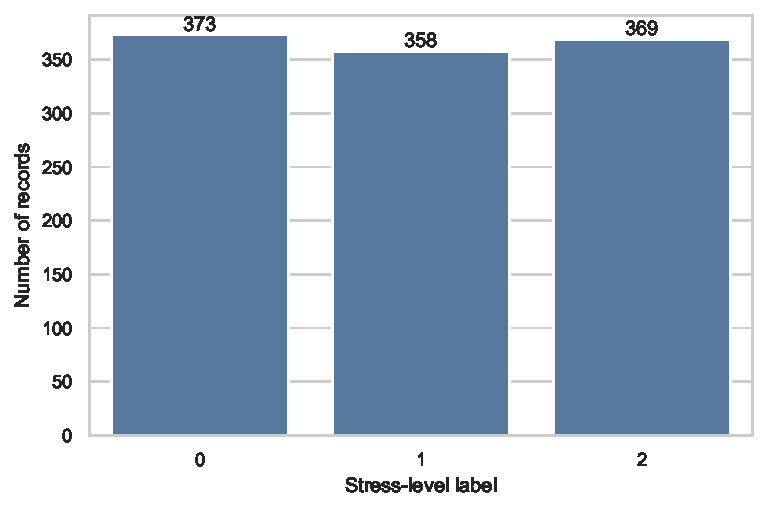
\includegraphics[width=.62\linewidth]{class_distribution.pdf}
\caption{Distribution of the supplied stress-level labels. The classes are approximately balanced; labels are shown numerically because their semantic mapping is not documented in the supplied files.}
\label{fig:class}
\end{figure}

\subsection{Predictors and domain grouping}
The predictors were grouped according to their column names and the conceptual framework (Figure~\ref{fig:framework}): psychological (anxiety level, self-esteem, mental-health history, depression); physiological (headache, blood pressure, sleep quality, breathing problem); environmental (noise level, living conditions, safety, basic needs); academic (academic performance, study load, teacher--student relationship, future-career concerns); and social (social support, peer pressure, extracurricular activities, bullying). Each domain contains four variables. Table~\ref{tab:data} summarises their observed ranges.

\begin{figure}[t]
\centering
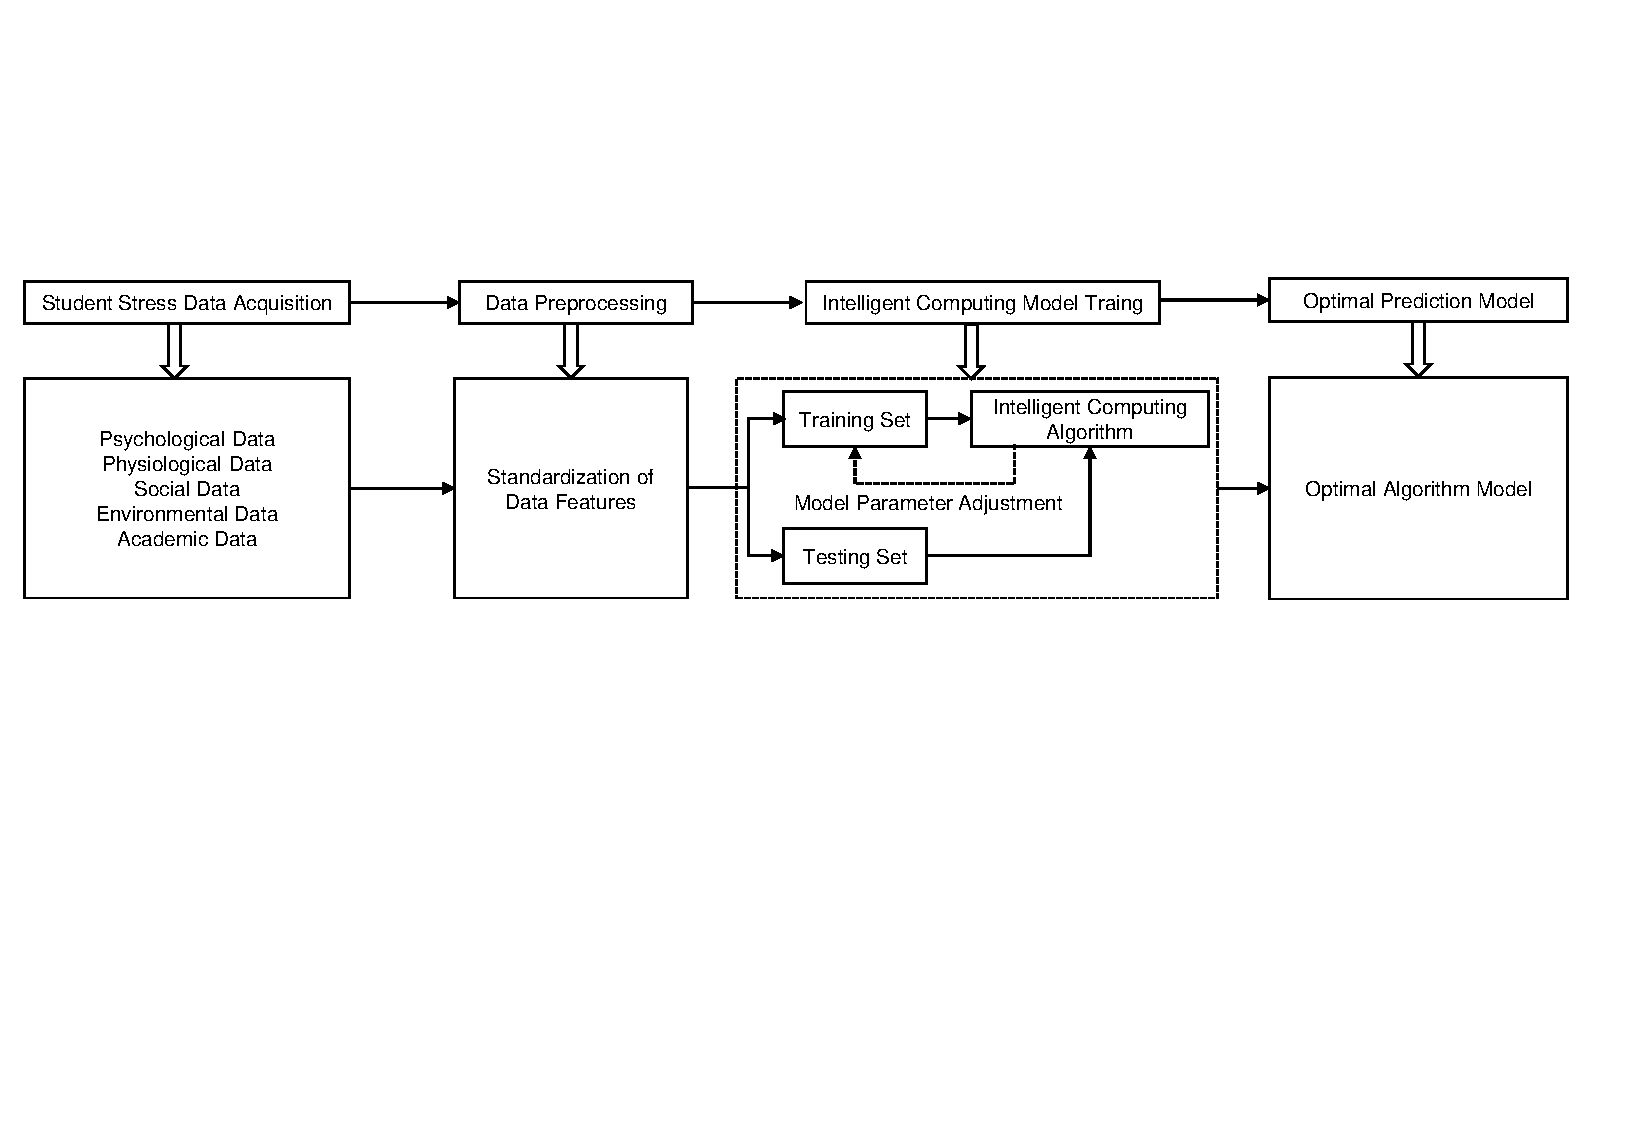
\includegraphics[width=.94\linewidth]{Framework.pdf}
\caption{Conceptual workflow used in this study: multidomain structured records are checked and standardised where required, models are trained under a common resampling protocol, and predictions are evaluated on held-out folds. The figure is conceptual and does not imply longitudinal sensing or multimodal raw signals.}
\label{fig:framework}
\end{figure}

\begin{table}[t]
\caption{Predictor domains and observed ranges in the supplied dataset.}
\label{tab:data}
\centering
\resizebox{\linewidth}{!}{%
\begin{tabular}{lll}
\toprule
Domain & Variables & Observed ranges \\
\midrule
Psychological & anxiety, self-esteem, history, depression & 0--21; 0--30; 0--1; 0--27 \\
Physiological & headache, blood pressure, sleep, breathing & 0--5; 1--3; 0--5; 0--5 \\
Environmental & noise, living, safety, basic needs & all 0--5 \\
Academic & performance, load, relationship, career & all 0--5 \\
Social & support, peer pressure, activities, bullying & 0--3; 0--5; 0--5; 0--5 \\
\bottomrule
\end{tabular}}
\end{table}

\subsection{Data audit and preprocessing}
All 21 columns are integer-valued and contain no missing entries. Consequently, no imputation or outlier deletion was performed. Removing observations solely because their values are extreme would be unjustified without the original scale definitions. StandardScaler was fitted inside each training fold for logistic regression, k-nearest neighbours (kNN), the radial-basis-function support vector machine (RBF-SVM), and the multilayer perceptron (MLP). Tree-based methods used the original numeric values. This fold-wise pipeline prevents validation-fold information from entering preprocessing.

The Pearson correlation matrix (Figure~\ref{fig:corr}) is descriptive. Since several predictors are ordinal, its magnitudes should not be interpreted as validated interval-scale effects.

\begin{figure}[t]
\centering
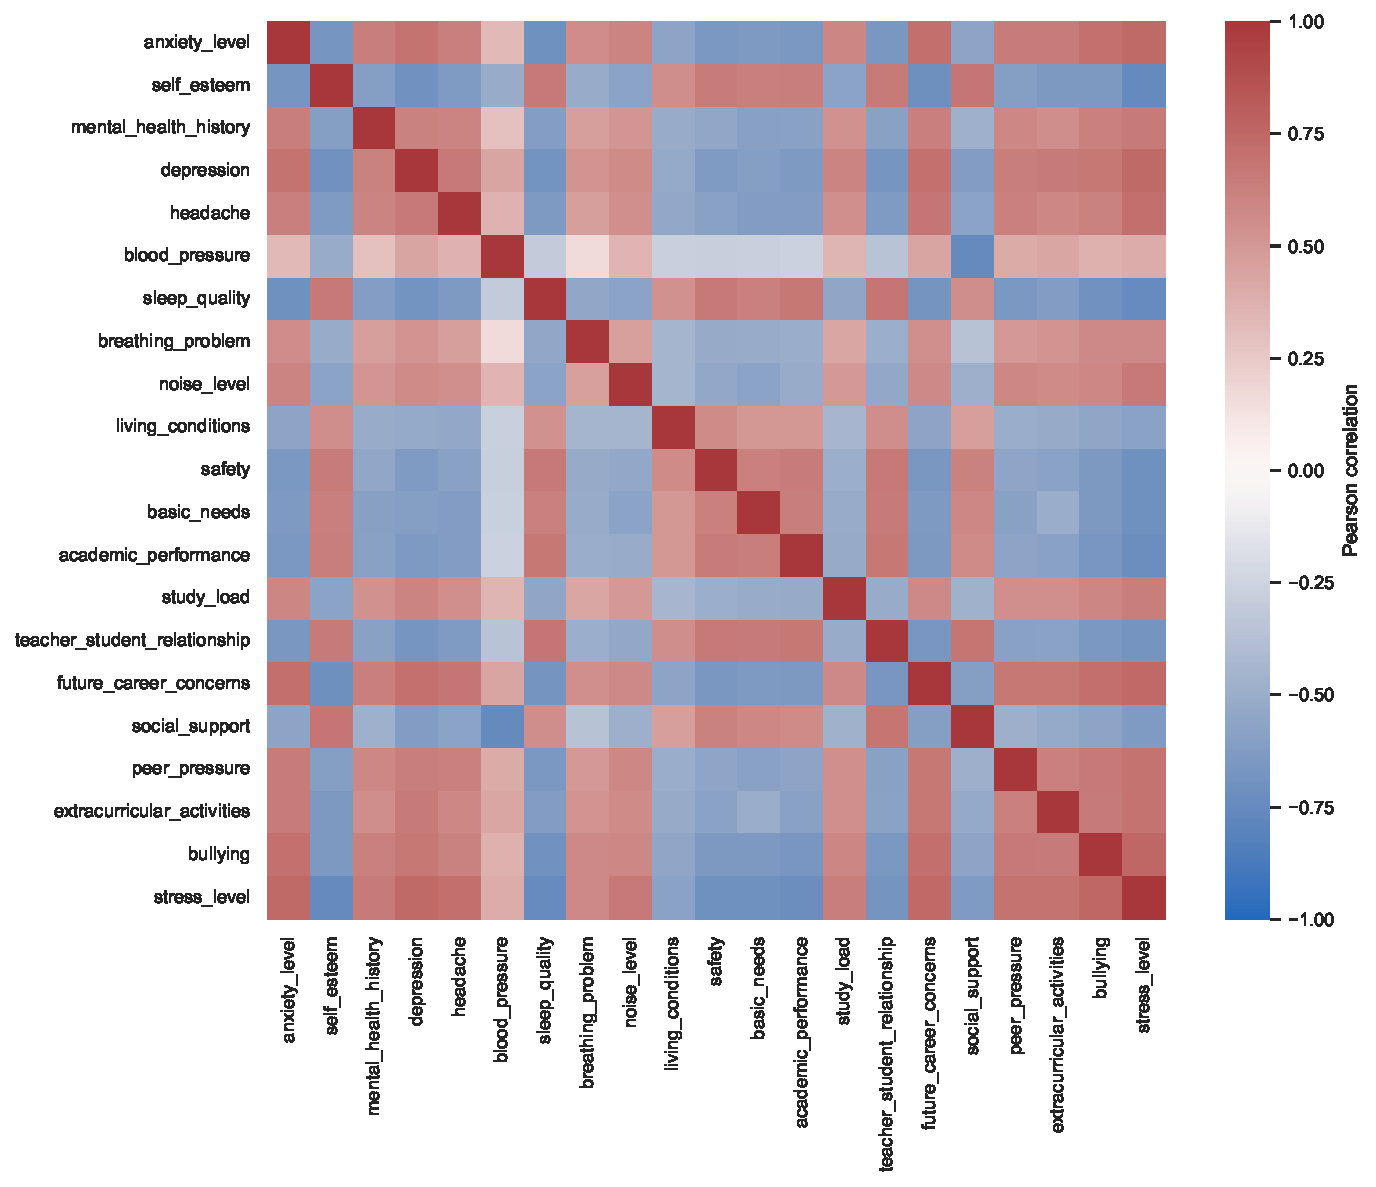
\includegraphics[width=.92\linewidth]{correlation_heatmap.pdf}
\caption{Pearson correlations among the 20 predictors and numeric stress label. The plot is used to screen redundancy, not to infer causal or clinical relationships.}
\label{fig:corr}
\end{figure}

\subsection{Models and evaluation protocol}
Eight classifiers were compared: multinomial logistic regression; kNN with $k=7$; RBF-SVM with $C=1$ and automatic scale-dependent $\gamma$; an unrestricted decision tree; random forest and Extra Trees ensembles with 500 trees; gradient boosting with default shrinkage and 100 estimators; and an MLP with hidden layers of 64 and 32 units and early stopping. Random seeds were fixed at 42 where supported. Implementations used scikit-learn~\cite{pedregosa2011}. These settings define a reproducible benchmark, not an exhaustive optimisation study.

Table~\ref{tab:modelsettings} places the principal implementation choices in the main text so that the comparison can be understood without consulting the supplement. The complete estimator specification is retained in Appendix~\ref{app:models}. No model-specific search was used to select the entries in the principal comparison; the separate random-forest grid is explicitly labelled as a sensitivity analysis.

\begin{table*}[t]
\caption{Main model and preprocessing specifications used in the matched comparison.}
\label{tab:modelsettings}
\centering
\resizebox{\textwidth}{!}{%
\begin{tabular}{llll}
\toprule
Model & Fold-wise preprocessing & Principal settings & Probability output/use \\
\midrule
Multinomial logistic regression & Standardisation & multinomial loss; $L_2$ penalty; fixed default regularisation & Native; calibration analysis \\
kNN & Standardisation & $k=7$; Euclidean neighbourhood & Neighbour proportions \\
RBF-SVM & Standardisation & $C=1$; scale-dependent $\gamma$ & Enabled for common evaluation \\
Decision tree & None & unrestricted depth; random state 42 & Leaf proportions \\
Random forest & None & 500 trees; random state 42 & Ensemble vote proportions \\
Extra Trees & None & 500 trees; random state 42 & Ensemble vote proportions \\
Gradient boosting & None & 100 estimators; default shrinkage; random state 42 & Native \\
MLP & Standardisation & hidden layers 64 and 32; early stopping; random state 42 & Softmax output \\
\bottomrule
\end{tabular}}
\end{table*}

Generalisation was estimated using five repeats of five-fold stratified cross-validation (25 held-out scores per model). All models were evaluated on identical splits. Accuracy and macro-averaged precision, recall, and F1 were calculated. For $K=3$ classes,
\begin{align}
\mathrm{Accuracy} &= \frac{\sum_{k=1}^{K}TP_k}{N},\\
P_{\mathrm{macro}} &= \frac{1}{K}\sum_{k=1}^{K}\frac{TP_k}{TP_k+FP_k},\\
R_{\mathrm{macro}} &= \frac{1}{K}\sum_{k=1}^{K}\frac{TP_k}{TP_k+FN_k},\\
F1_{\mathrm{macro}} &= \frac{1}{K}\sum_{k=1}^{K}\frac{2P_kR_k}{P_k+R_k}.
\end{align}
Macro averaging gives each label equal weight. Reported uncertainty is the sample standard deviation across the 25 held-out folds; it is not a confidence interval because repeated folds are not independent.

\subsection{Ablation, parameter sensitivity, and interpretation}
Domain-restricted ablation retrained the best comparison model using each four-feature domain alone, under the same repeated cross-validation splits. Random-forest sensitivity varied the number of trees in $\{50,100,200,500,800\}$ and maximum depth in $\{5,10,20,\text{unrestricted}\}$ using one fixed stratified five-fold split. Finally, the best model's feature relevance was estimated by permutation importance on each held-out fold: a predictor was shuffled 20 times, and the decrease in macro-F1 was aggregated across folds. This assesses predictive reliance conditional on correlated predictors; it does not measure causality.

\subsection{Uncertainty, calibration, and sample-size analysis}
The repeated-fold standard deviation characterises variation across resampled test folds but is not a conventional confidence interval. To provide an additional uncertainty summary for the fixed five-fold out-of-fold predictions, 2,000 nonparametric bootstrap samples of the 1,100 prediction--label pairs were drawn with replacement. Percentile limits at 2.5\% and 97.5\% were reported for accuracy and macro-F1. This bootstrap conditions on the fitted out-of-fold predictions and therefore does not incorporate uncertainty about data collection or transport to a new institution.

Probability quality was examined in a one-versus-rest manner for each label. For label $k$, the Brier score was
\begin{equation}
B_k=\frac{1}{N}\sum_{i=1}^{N}(p_{ik}-\mathbf{1}[y_i=k])^2,
\end{equation}
where $p_{ik}$ denotes the out-of-fold probability assigned to label $k$ and $\mathbf{1}[\cdot]$ is the indicator function. Reliability diagrams grouped predictions into eight equal-frequency bins and compared the mean predicted probability with the observed class frequency. Calibration curves were treated as descriptive because only 1,100 records were available.

Learning curves were calculated for the leading model using ten training-set fractions between 10\% and 100\% of each training fold. At each fraction, training and validation macro-F1 were averaged across the same fixed five-fold split. The separation between these curves indicates whether error is more consistent with insufficient model capacity, overfitting, or limited sample size.

\subsection{Reproducibility controls}
The analysis script performs data loading, integrity checks, model construction, resampling, metric calculation, tabular export, and figure generation in a single executable workflow. Preprocessing is encapsulated in a pipeline and is refitted within each training fold. Random-state values are fixed where the estimator exposes such a parameter. Results are saved as comma-separated files before being transcribed into the manuscript, which provides an auditable connection between the data and each reported number. The supplied CSV is never overwritten or cleaned in place.

Four design choices limit researcher degrees of freedom. First, macro-F1 was declared the principal class-balanced metric before model comparison. Second, identical splits were used across algorithms. Third, the comparison table reports all tested models rather than only the best result. Fourth, the parameter grid is presented in full in Appendix~\ref{app:parameters}. These controls do not replace external replication, but they reduce selective reporting within the available dataset.

\section{Results}\label{sec:results}
\subsection{Comparative performance}
Table~\ref{tab:comparison} reports the repeated-validation results. Multinomial logistic regression achieved the highest mean macro-F1 (0.8866) and, together with gradient boosting, the highest accuracy (0.8864). Differences among the top three models were smaller than their fold-to-fold standard deviations. Thus, the experiment does not support a claim that the most complex model is superior.

\begin{table*}[t]
\caption{Five-times repeated five-fold stratified cross-validation. Values are mean $\pm$ standard deviation across 25 held-out folds.}
\label{tab:comparison}
\centering
\resizebox{\textwidth}{!}{%
\begin{tabular}{lcccc}
\toprule
Model & Accuracy & Macro-precision & Macro-recall & Macro-F1 \\
\midrule
Multinomial logistic regression & \textbf{0.8864}$\pm$0.0169 & \textbf{0.8886}$\pm$0.0166 & \textbf{0.8863}$\pm$0.0169 & \textbf{0.8866}$\pm$0.0169 \\
Gradient boosting & \textbf{0.8864}$\pm$0.0193 & 0.8875$\pm$0.0190 & \textbf{0.8863}$\pm$0.0193 & 0.8863$\pm$0.0193 \\
Decision tree & 0.8844$\pm$0.0208 & 0.8863$\pm$0.0212 & 0.8843$\pm$0.0207 & 0.8844$\pm$0.0208 \\
Random forest & 0.8787$\pm$0.0195 & 0.8823$\pm$0.0185 & 0.8786$\pm$0.0194 & 0.8790$\pm$0.0193 \\
Extra Trees & 0.8775$\pm$0.0178 & 0.8811$\pm$0.0168 & 0.8773$\pm$0.0178 & 0.8778$\pm$0.0176 \\
RBF-SVM & 0.8755$\pm$0.0177 & 0.8829$\pm$0.0156 & 0.8752$\pm$0.0178 & 0.8764$\pm$0.0173 \\
MLP & 0.8753$\pm$0.0184 & 0.8774$\pm$0.0181 & 0.8754$\pm$0.0186 & 0.8753$\pm$0.0184 \\
kNN & 0.8645$\pm$0.0218 & 0.8703$\pm$0.0212 & 0.8652$\pm$0.0218 & 0.8649$\pm$0.0217 \\
\bottomrule
\end{tabular}}
\end{table*}

A separate five-fold out-of-fold prediction run for logistic regression produced the confusion matrix in Figure~\ref{fig:cm}. Correct predictions numbered 331/373 for label 0, 318/358 for label 1, and 331/369 for label 2. Errors were distributed across all class pairs rather than concentrated in one minority class.

Figure~\ref{fig:modelcomparison} visualises the same fold-level macro-F1 means and standard deviations. Its purpose is to show effect magnitude and uncertainty together: the ordering is visible, but the extensive overlap cautions against declaring a practically meaningful winner from small mean differences.

\begin{figure}[t]
\centering
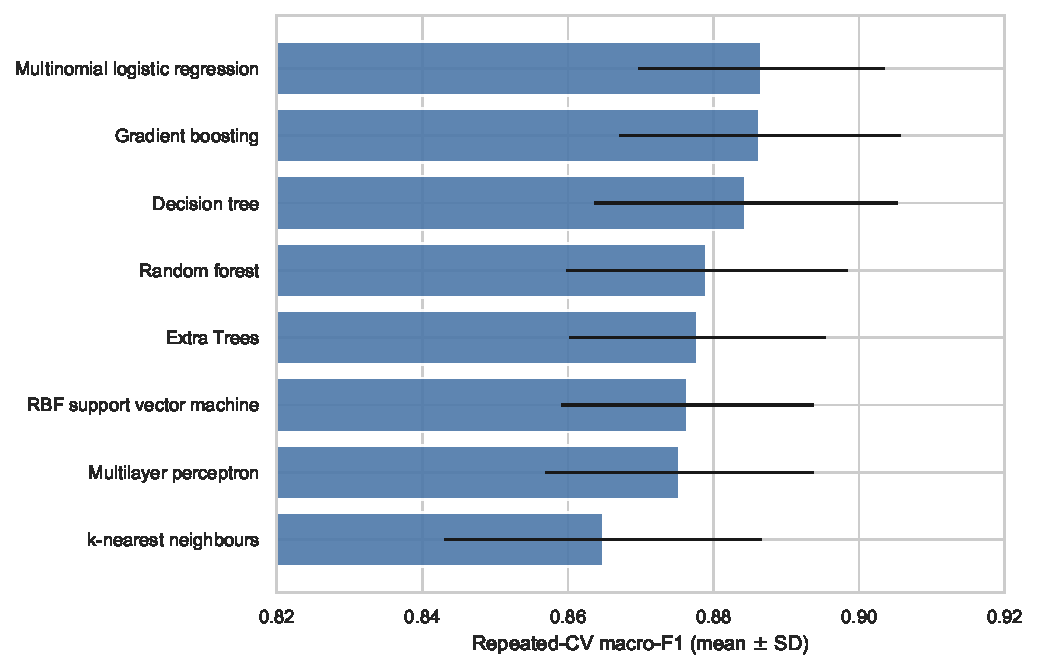
\includegraphics[width=.88\linewidth]{model_comparison.pdf}
\caption{Matched comparison of eight classifiers under five-times repeated five-fold stratified cross-validation. Bars show mean macro-F1 and error bars show one standard deviation across 25 held-out folds.}
\label{fig:modelcomparison}
\end{figure}

\begin{figure}[t]
\centering
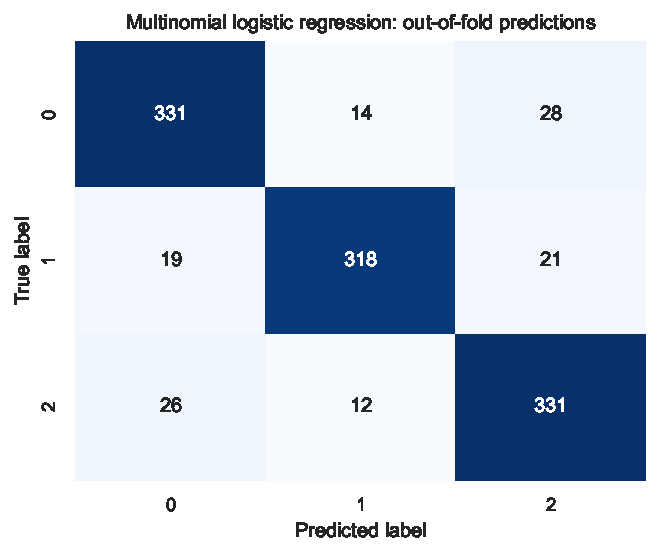
\includegraphics[width=.67\linewidth]{confusion_matrix.pdf}
\caption{Out-of-fold confusion matrix for multinomial logistic regression using one fixed five-fold stratified split. Every record is predicted by a model that did not train on that record.}
\label{fig:cm}
\end{figure}

\subsection{Class-specific performance and uncertainty}
The fixed out-of-fold predictions enable a closer examination of each encoded label (Table~\ref{tab:classmetrics}). Label 1 had the highest precision (0.9244) and F1 (0.9060), whereas labels 0 and 2 both had F1 0.8838. Recall ranged only from 0.8874 to 0.8970. The narrow range shows that the aggregate score was not produced by sacrificing one class, although this conclusion applies only to the three numeric labels and not to unobserved demographic subgroups.

\begin{table}[t]
\caption{Per-class metrics from the fixed five-fold out-of-fold predictions.}
\label{tab:classmetrics}
\centering
\begin{tabular}{lrrrr}
\toprule
Label & Precision & Recall & F1 & Support \\
\midrule
0 & 0.8803 & 0.8874 & 0.8838 & 373 \\
1 & 0.9244 & 0.8883 & 0.9060 & 358 \\
2 & 0.8711 & 0.8970 & 0.8838 & 369 \\
\midrule
Macro average & 0.8919 & 0.8909 & 0.8912 & 1,100 \\
\bottomrule
\end{tabular}
\end{table}

The point accuracy for this fixed out-of-fold run was 0.8909, with a bootstrap percentile interval of 0.8727--0.9091. Macro-F1 was 0.8912, with a percentile interval of 0.8731--0.9088. These intervals quantify sampling variation in the existing record-level predictions; they do not account for possible clustering by school, repeated observations of the same student, measurement error, or dataset construction, none of which can be identified from the supplied metadata.

\subsection{Domain-restricted ablation}
As shown in Table~\ref{tab:ablation}, each domain alone retained considerable predictive information. The physiological subset yielded a macro-F1 of 0.8884, marginally above the 20-feature result, whereas the academic subset yielded 0.8634. Because the difference is small relative to cross-fold variability and domains are correlated, this result should be interpreted as evidence of redundancy, not proof that other domains are unimportant.

\begin{table}[t]
\caption{Domain-restricted logistic-regression analysis under repeated cross-validation.}
\label{tab:ablation}
\centering
\begin{tabular}{lcc}
\toprule
Feature set & No. features & Macro-F1 \\
\midrule
Physiological & 4 & \textbf{0.8884}$\pm$0.0195 \\
All domains & 20 & 0.8866$\pm$0.0169 \\
Environmental & 4 & 0.8750$\pm$0.0207 \\
Psychological & 4 & 0.8733$\pm$0.0199 \\
Social & 4 & 0.8690$\pm$0.0199 \\
Academic & 4 & 0.8634$\pm$0.0191 \\
\bottomrule
\end{tabular}
\end{table}

\subsection{Leave-one-domain-out robustness}
The domain-only experiment asks whether a small group is sufficient; the complementary leave-one-domain-out analysis asks whether that group is necessary in the presence of the other 16 predictors. Results are reported in Table~\ref{tab:leaveout}. Removing physiological variables caused the largest decline, reducing macro-F1 from 0.8866 to 0.8738. Removing the academic domain slightly increased the mean to 0.8897, while removing psychological, environmental, or social variables produced changes smaller than the repeated-fold dispersion.

\begin{table}[t]
\caption{Leave-one-domain-out logistic-regression robustness analysis.}
\label{tab:leaveout}
\centering
\begin{tabular}{lcc}
\toprule
Omitted domain & Remaining features & Macro-F1 \\
\midrule
Academic & 16 & 0.8897$\pm$0.0191 \\
Psychological & 16 & 0.8870$\pm$0.0191 \\
Environmental & 16 & 0.8863$\pm$0.0166 \\
Social & 16 & 0.8855$\pm$0.0213 \\
Physiological & 16 & 0.8738$\pm$0.0174 \\
\bottomrule
\end{tabular}
\end{table}

Taken together, the two ablations support a limited statement: physiological coding carries concentrated predictive information in this dataset, and the remaining domains contain overlapping signals. The analyses do not show that a physiological-only instrument would remain accurate in another student population. In particular, the dominant blood-pressure variable has only three values and may have been used directly or indirectly when the public labels were constructed.

Figure~\ref{fig:domainrobustness} aligns the two ablation directions on one scale. A domain can be sufficient on its own yet dispensable when correlated alternatives are available. The physiological domain is distinctive because it combines the strongest standalone result with the largest deterioration after omission; the academic domain shows the converse pattern.

\begin{figure}[t]
\centering
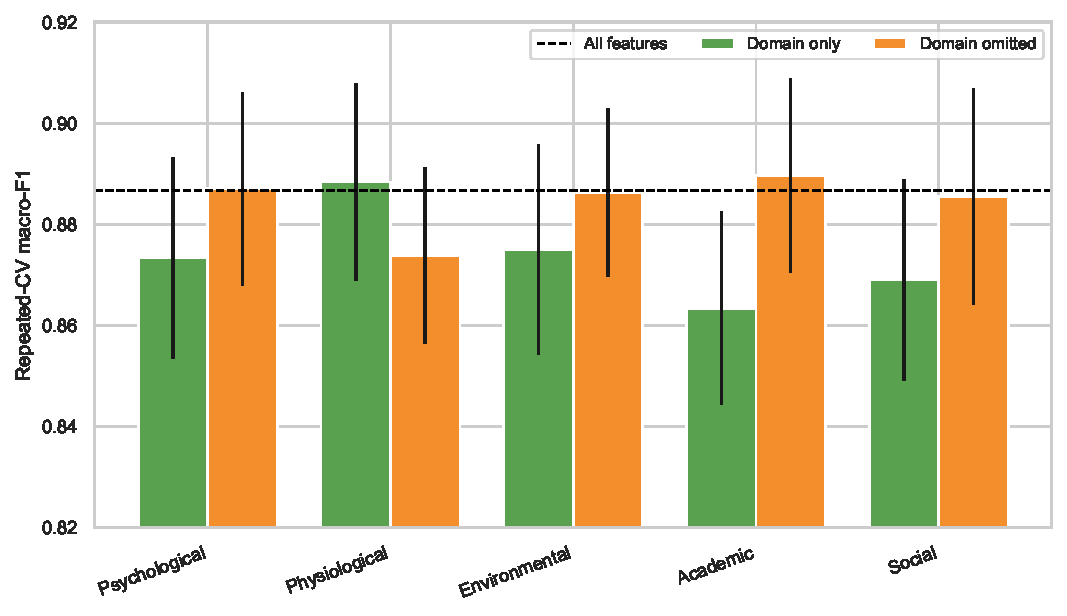
\includegraphics[width=.98\linewidth]{domain_robustness.pdf}
\caption{Complementary domain analyses for logistic regression. ``Domain only'' uses four predictors; ``domain omitted'' uses the remaining 16. The dashed line is the all-feature macro-F1. Error bars show repeated-fold standard deviations.}
\label{fig:domainrobustness}
\end{figure}

\subsection{Parameter sensitivity}
Across the 20 random-forest configurations, mean macro-F1 ranged from 0.8705 to 0.8858. The highest tested value occurred with 50 trees and maximum depth 5 (0.8858$\pm$0.0054), while increasing the ensemble to 500 or 800 trees did not consistently improve performance. This narrow range and non-monotonic pattern indicate that the main comparison is not explained simply by an insufficient number of trees. Since the same folds were used to inspect all settings, the maximum is descriptive and must not be treated as an unbiased tuned-model estimate.

\begin{figure}[t]
\centering
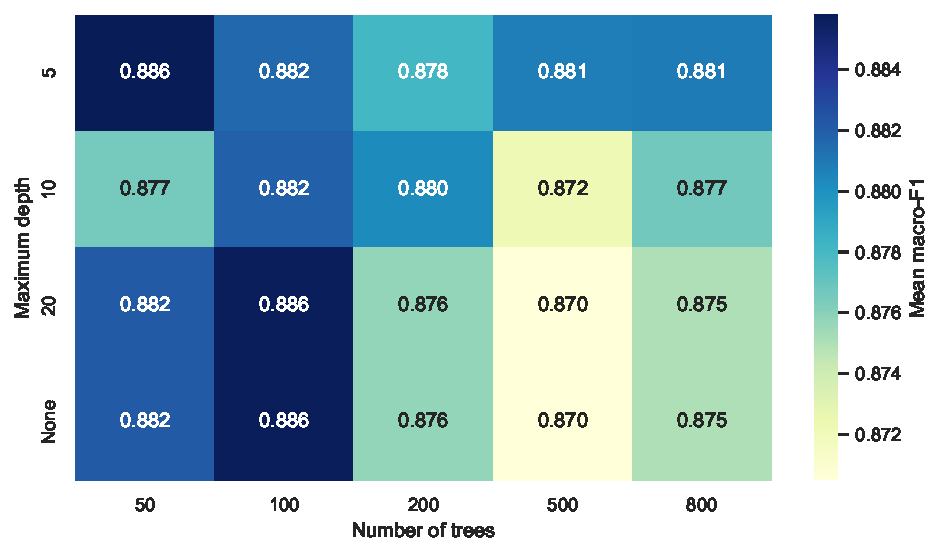
\includegraphics[width=.82\linewidth]{rf_sensitivity_heatmap.pdf}
\caption{Random-forest parameter sensitivity across the complete 20-setting grid. Cells report mean five-fold macro-F1. The limited colour range makes the small, non-monotonic differences visible; it does not represent nested hyperparameter optimisation.}
\label{fig:rfsensitivity}
\end{figure}

\subsection{Predictive feature relevance}
Cross-validated permutation importance (Figure~\ref{fig:importance}) showed the largest macro-F1 decrease after permuting blood pressure, followed by social support. Most remaining variables produced small conditional decreases. This concentration helps explain why a four-variable physiological model performed competitively. However, importance can be redistributed among correlated or redundantly encoded variables and may reflect label-generation rules in the source dataset.

\begin{figure}[t]
\centering
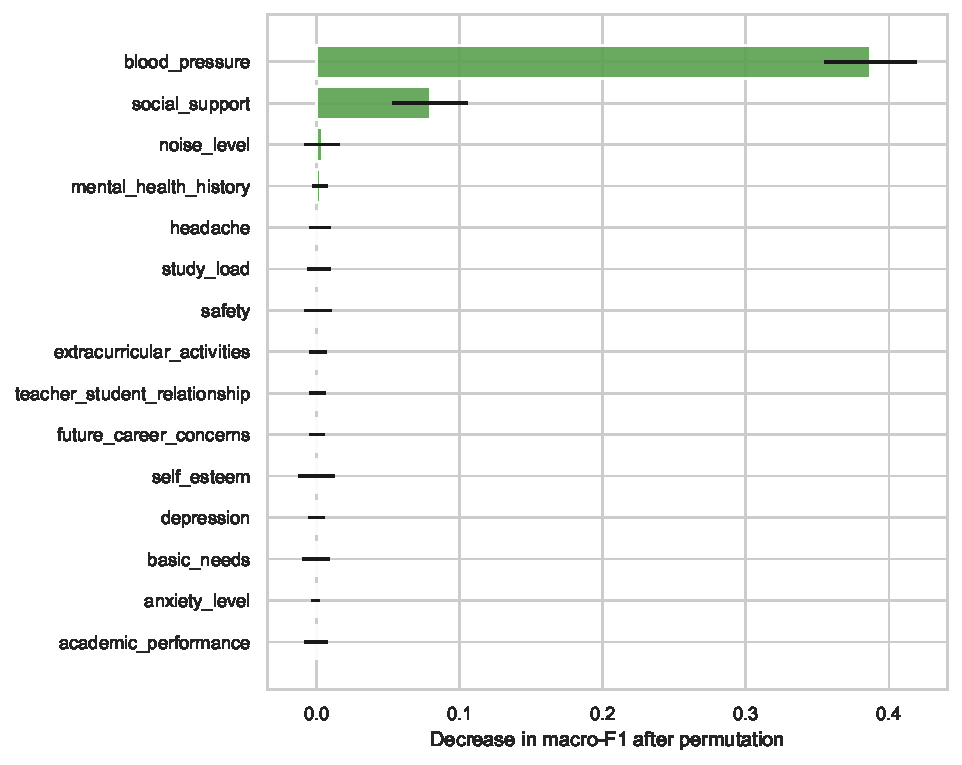
\includegraphics[width=.8\linewidth]{permutation_importance.pdf}
\caption{Cross-validated permutation importance for the logistic-regression model. Bars show the mean decrease in held-out macro-F1; error bars show the standard deviation across 100 fold--repeat permutations (20 repeats in each of five folds). Negative or near-zero values indicate no stable conditional contribution under this model.}
\label{fig:importance}
\end{figure}

\subsection{Learning behaviour}
Figure~\ref{fig:learning} shows the learning curve for multinomial logistic regression. At the smallest training size, the training estimate was high while validation performance was lower and more variable. The gap narrowed as training size increased, with validation macro-F1 approaching the repeated-validation result. The validation curve had not become completely flat at the largest available size, so additional representative records may still reduce uncertainty. At the same time, the small terminal train--validation gap provides no evidence that adding model capacity alone would yield a major improvement.

\begin{figure}[p]
\centering
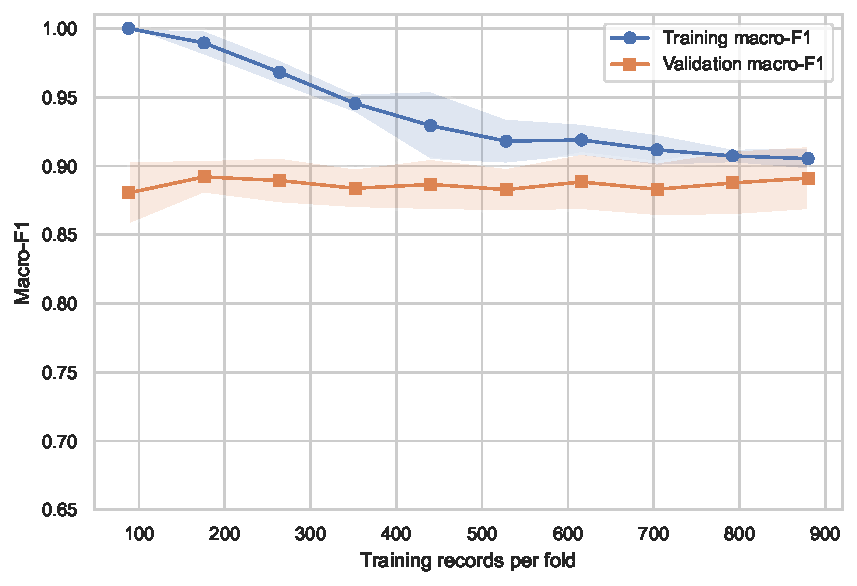
\includegraphics[width=.78\linewidth]{learning_curve.pdf}
\caption{Learning curve for multinomial logistic regression. Lines show five-fold means and shaded regions show one standard deviation. Training size is the number of records available within each training fold.}
\label{fig:learning}
\end{figure}

\subsection{Probability calibration}
The one-versus-rest Brier scores were 0.0511, 0.0429, and 0.0512 for labels 0, 1, and 2, respectively. Label 1 therefore had the lowest mean squared probability error, consistent with its higher class-specific F1. Figure~\ref{fig:calibration} compares binned predicted and observed frequencies. The curves broadly follow the identity line but deviate in some bins, especially where observations are sparse. These results do not justify fixed decision thresholds for practice. External recalibration would be necessary if class prevalence or measurement procedures changed.

\begin{figure}[p]
\centering
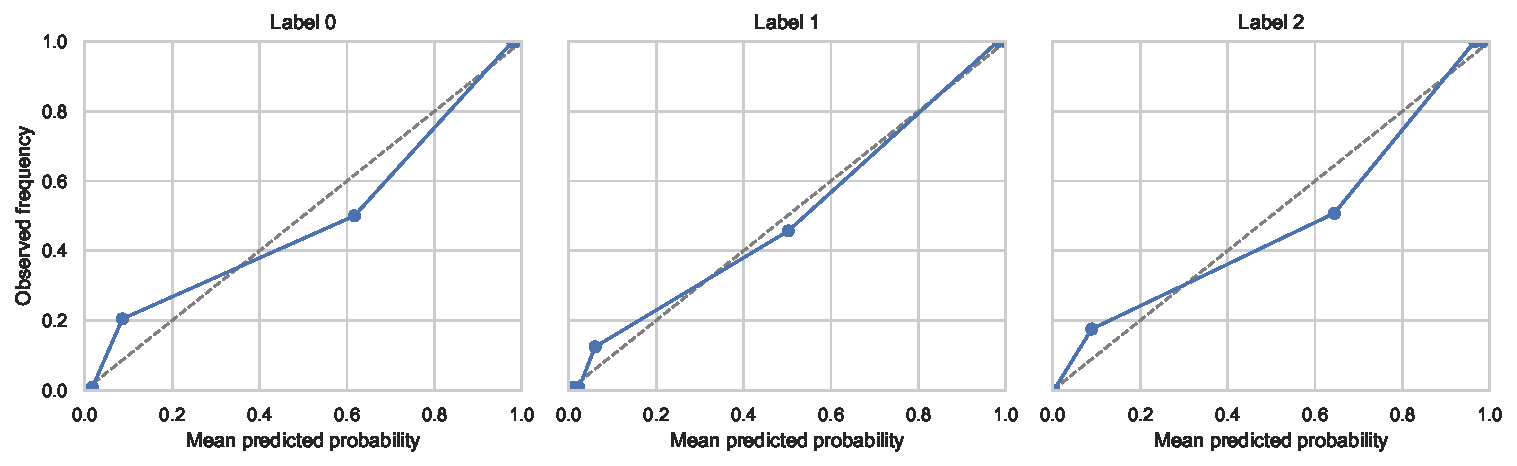
\includegraphics[width=.98\linewidth]{calibration_curves.pdf}
\caption{One-versus-rest reliability diagrams based on fixed five-fold out-of-fold probabilities and eight equal-frequency bins. The dashed diagonal represents ideal calibration.}
\label{fig:calibration}
\end{figure}

\section{Discussion}\label{sec:discussion}
The principal finding is that all eight classifiers achieved broadly similar performance, with multinomial logistic regression providing the strongest macro-F1 and gradient boosting tying its accuracy. For this dataset, complexity was not rewarded. A plausible explanation is that the target is encoded by a relatively simple combination of a few variables, while other domains duplicate similar information. The strong performance of domain-restricted models reinforces this interpretation.

The physiological subset's slight advantage over the complete feature set should not be translated into a clinical claim that physiology causes or dominates student stress. Blood pressure has only three encoded values, and the supplied documentation does not clarify whether it represents measured pressure, an ordinal category, or a derived score. Likewise, social support may be protective in substantive studies, but the present analysis only establishes its usefulness for predicting the supplied label. Dataset documentation and external validation are prerequisites for substantive interpretation.

The results have two practical implications. First, transparent linear baselines should accompany complex intelligent-computing models on small structured datasets. Second, a future data-collection instrument may be simplified only after confirming that the apparent redundancy persists in independently sampled students and that reduced features do not impair subgroup performance. A predictive model is not a diagnostic instrument and should not trigger interventions without professional review, informed consent, privacy protections, and assessment of potential harms.

\subsection{Why the linear model was competitive}
The comparison challenges the assumption that an ``intelligent computing'' contribution must depend on a deep architecture. An MLP can represent nonlinear interactions, an RBF-SVM can form curved decision boundaries, and tree ensembles can partition the feature space into many local regions. None produced a stable advantage over multinomial logistic regression. Three non-exclusive explanations are consistent with the evidence.

First, the encoded outcome may be approximately linearly separable after standardisation. This is particularly plausible if the public dataset was created by thresholding or combining questionnaire scores. Second, correlated variables allow a linear model to approximate nonlinear-looking associations through multiple weighted inputs. Third, the sample of 1,100 records may be too small to estimate flexible boundaries reliably, so the lower variance of a linear classifier offsets the additional bias. The learning curve supports the third explanation only partially: validation performance continued to improve with sample size, but the final training--validation gap was modest.

The practical lesson is methodological rather than algorithm-specific. A model class should be justified by observed gains under a leakage-resistant protocol, not by its novelty or capacity. When a transparent baseline performs equally well, it offers easier auditing, more stable optimisation, and a clearer route to calibration. This does not prove that deep learning is unsuitable for student stress research; it indicates that deep learning is not supported for this small, cross-sectional, fully tabular benchmark.

\subsection{Relation to recent student-stress studies}
Recent student-focused studies demonstrate the breadth of the field rather than a single settled modelling recipe. Multimodel tabular analyses combine lifestyle, academic, and social factors~\cite{defilippis2024}; fuzzy approaches represent gradual well-being group membership~\cite{han2023}; passive smartphone sensing captures behavioural signals unavailable to a cross-sectional questionnaire~\cite{shvetcov2024}; and systematic reviews document continuing heterogeneity in both labels and evaluation practices~\cite{daza2023,cruz2025,humayun2025}. The present results complement these studies by holding the dataset, folds, preprocessing boundaries, and metrics constant across eight estimators.

The numerical scores should not be ranked directly against results from those studies. A passive-sensing forecast over future days is a different target from concurrent three-class label reconstruction, and a clinically validated scale is different from an undocumented public benchmark label. Sample composition and splitting unit also matter: record-wise random validation can be optimistic if multiple records originate from the same person, class, institution, or time period. Because the supplied metadata do not expose those structures, repeated stratification is the strongest defensible internal evaluation here, but it cannot resolve possible hidden dependence. The paper's contribution is therefore the completeness and auditability of evidence within one benchmark, not a claim of state-of-the-art clinical prediction.

\subsection{Triangulating the ablation results}
Domain-only and leave-one-domain-out analyses answer different questions and should be interpreted together. The physiological domain was nearly sufficient by itself and its removal caused the largest deterioration. Conversely, the academic domain was the weakest standalone subset and its removal slightly improved mean performance. If only the first analysis were reported, one might incorrectly conclude that academic information has no value; if only the second were reported, one might overlook that it remains individually predictive. Their combination indicates redundancy: several domains can approximate the label, but the physiological coding contains information that is less fully replaced by other variables.

This pattern raises a data-quality question. In real student populations, stress is unlikely to be reducible to a three-level blood-pressure code. The observed concentration may therefore reflect construct overlap, a deterministic label-generation rule, or synthetic/curated data. Without the original codebook and recruitment protocol, these alternatives cannot be distinguished. External data should specifically test whether the blood-pressure effect persists after controlling for measurement setting, medication, health status, and repeated measurements.

\subsection{Interpretability and causal boundaries}
Permutation importance measures the decline in held-out performance when one column is disrupted. It is preferable here to reporting training-set coefficients alone because it evaluates the complete fitted pipeline on unseen folds. Nevertheless, it has three limitations. Correlated predictors can substitute for one another, reducing their measured importance; a variable can be predictively important because of bias or leakage; and the magnitude depends on the chosen metric and model. The importance plot should therefore be read as a model-audit tool rather than a ranking of intervention targets.

No result estimates the effect of changing a predictor. Increasing a social-support score, improving sleep, or reducing study load may be beneficial in practice, but the present data cannot quantify those effects. Intervention claims would require longitudinal or experimental designs, temporal ordering, measurement validation, and adjustment for confounding. Similarly, the model cannot distinguish transient stress responses from persistent or clinically significant conditions.

\subsection{Calibration and decision support}
Classification accuracy answers whether the most likely label is correct; calibration asks whether predicted probabilities correspond to observed frequencies. Both are necessary if probabilities are used to prioritise follow-up. The relatively low Brier scores and approximately diagonal reliability curves are encouraging internally, but apparent calibration can degrade substantially when prevalence, survey administration, or institutional context changes. Recalibration on an external validation cohort would therefore be mandatory.

Even a calibrated model does not specify an appropriate action threshold. Threshold selection should reflect the relative costs of missed support needs, unnecessary follow-up, privacy intrusion, and resource constraints. Those costs were not present in the supplied files. A responsible deployment study should define a prospective pathway in which the model augments, rather than replaces, student self-report and professional judgement; it should also provide an opt-out mechanism and a procedure for contesting or correcting data.

\subsection{Implications for data collection}
The present audit shows that complete numeric tables are not equivalent to well-documented research data. Future collection should record the sampling frame, recruitment rate, school or programme, observation date, age range, gender and other fairness-relevant attributes where ethically justified, questionnaire names, item wording, scoring direction, missingness reasons, and whether multiple rows can represent the same student. A pre-specified protocol should distinguish predictors available before prediction from variables collected simultaneously with or after the outcome.

Longitudinal data would enable forecasting rather than concurrent classification. A useful design might establish a baseline, collect repeated weekly or monthly measurements, and define a prediction horizon. Grouped splitting by participant and temporal splitting by date would then prevent the same person's history or future information from leaking into evaluation. Independent institutional validation should be planned before deployment rather than treated as an optional final step.

\subsection{From benchmark to prospective deployment}
Moving from an offline benchmark to student support would require a prospective protocol with a frozen model, an independently defined outcome, a prediction horizon, and a documented response pathway. Recent work on student recommendation engines and digital mental-health services emphasises that prediction must connect to existing care and institutional processes~\cite{velmovitsky2025,pryss2025}. A pilot should consequently evaluate uptake, false-alert workload, time to appropriate support, student understanding, and adverse consequences in addition to discrimination.

The model should first be externally evaluated without retraining, followed by recalibration or updating only when prespecified criteria are met. Reporting should follow TRIPOD+AI, while risk of bias and applicability should be assessed with PROBAST+AI~\cite{collins2024,moons2025}. Any user interface should present uncertainty and the source of input data, avoid diagnostic language, and permit human review. These requirements are deliberately outside the claims of the current experiment, but stating them clarifies what evidence is still needed before real-world use.

\subsection{Ethical, privacy, and governance considerations}
Student mental-health prediction involves sensitive data and power asymmetries. Students may feel compelled to participate when collection is linked to teaching platforms or institutional services. Data minimisation, transparent purpose limitation, secure retention, and role-based access are therefore essential. Predictions should not be used for grading, disciplinary action, admissions, insurance, or other high-impact decisions unrelated to support.

Fairness cannot be assessed in the supplied dataset because demographic and institutional group variables are absent. This absence protects some privacy but prevents evaluation of differential error. A future study should define which subgroup analyses are scientifically and ethically appropriate, ensure adequate sample sizes, report uncertainty rather than unstable point estimates, and involve students and counselling professionals in determining acceptable uses. Model monitoring should address distribution shift, calibration drift, complaint handling, and retirement criteria.

\subsection{Limitations and threats to validity}
This study has several important limitations. (1) The public file lacks sampling, demographic, institutional, temporal, consent, and ethics metadata; representativeness cannot be assessed. (2) Definitions and psychometric evidence for the predictors and outcome are unavailable. (3) The data are cross-sectional, precluding causal and temporal claims. (4) Repeated cross-validation estimates internal consistency on one dataset, not generalisation across schools, regions, or years. (5) No sensitive demographic attributes are available, so fairness and subgroup calibration cannot be evaluated. (6) Parameter sensitivity was limited to a random-forest grid and was not nested within an outer validation loop. (7) Feature importance is model- and distribution-dependent. (8) The near-equivalence of several models requires statistical comparison on independent cohorts before ranking them definitively.

An independent cohort was not available in the supplied materials. The study is therefore presented as a reproducible comparative analysis with internal evaluation. Consistent with contemporary prediction-model guidance~\cite{collins2024,van2024evaluation,moons2025}, no deployment or clinical-validity claim is made, and external evaluation remains the principal next step.

\subsection{Priorities for future research}
The most important next step is not testing another algorithm on the same records; it is validating the construct and the data-generation process. A staged programme is recommended. Stage 1 should recover the codebook, provenance, and licensing information. Stage 2 should replicate the analysis on an independently collected cohort using frozen preprocessing and model specifications. Stage 3 should assess temporal stability, calibration, and subgroup errors. Stage 4 may compare parsimonious and expanded instruments prospectively. Only after these stages should a decision-support pilot examine workflow integration, user understanding, and unintended consequences.

Further methodological work could use ordinal models if labels 0--2 are confirmed to have ordered meanings, multilevel models if students are clustered within institutions, and survival or recurrent-event models if longitudinal outcomes become available. Missing-data mechanisms should be documented and handled within resampling. Nested cross-validation or a locked external test set should be used for substantive hyperparameter optimisation. Decision-curve analysis may be appropriate once clinically or educationally meaningful consequences and thresholds are defined.

\section{Conclusion}\label{sec:conclusion}
This reproducible comparative study evaluated eight classifiers for three-class student stress-level prediction from 20 variables spanning five psychological, physiological, environmental, academic, and social domains. Multinomial logistic regression achieved macro-F1 0.8866$\pm$0.0169, while more complex models did not provide a reliable advantage. Complementary domain analyses and cross-validated permutation importance made the comparison interpretable by revealing extensive redundancy and concentrated predictive reliance, particularly on blood-pressure coding and social support. The findings support an internally validated multidimensional prediction baseline rather than a clinical tool. Reliable real-world use requires authoritative variable definitions, documented sampling and ethics, independent external validation, calibration, and fairness assessment.

\section*{Acknowledgement}
This work was supported in part by the China Postdoctoral Science Foundation (Grant No. 2025M771665).

\section*{Data and Code Availability}
The public dataset is available from the \href{https://www.kaggle.com/datasets/rxnach/student-stress-factors-a-comprehensive-analysis}{Kaggle Student Stress Factors repository}. The complete executable analysis script, fold-level scores, aggregate tables, and figure source data are included as supplementary files accompanying this manuscript. The analysis reads the raw CSV without modifying it.

\section*{Ethics Statement}
This study is a secondary computational analysis of an openly accessible, de-identified benchmark dataset. The authors had no contact with participants, received no identifiable information, and conducted no new recruitment or intervention. Institutional review board approval and additional informed consent were therefore not applicable to the analyses reported here. The absence of primary-source ethics and recruitment metadata is explicitly treated as a limitation and precludes clinical or population-level interpretation.

\section*{Conflict of Interest}
The authors declare no known financial or personal relationships that could have influenced the work reported in this paper.

\section*{Author Contributions}
Heng Wu: Conceptualization, methodology, software, formal analysis, visualization, writing---original draft, and writing---review and editing. Zhiming Yan: Conceptualization, supervision, validation, resources, funding acquisition, and writing---review and editing. Both authors approved the final manuscript.

\appendix
\clearpage
\section{Complete Descriptive Audit}\label{app:descriptive}
Table~\ref{tab:descriptive-full} reports the complete univariate audit used before modelling. Counts equal 1,100 for every variable and no missing values were detected. The table deliberately reports observed values without assigning questionnaire units or clinical cut points that are absent from the source documentation. Several columns have narrow integer ranges and should be treated as encoded ordinal variables unless the authors recover evidence supporting interval-scale interpretation.

{\small
\begin{longtable}{p{3.4cm}rrrrrr}
\caption{Complete descriptive statistics for predictors and outcome.}\label{tab:descriptive-full}\\
\toprule
Variable & Mean & SD & Min & Median & Max & Missing \\
\midrule
\endfirsthead
\multicolumn{7}{c}{\tablename\ \thetable\ -- continued}\\
\toprule
Variable & Mean & SD & Min & Median & Max & Missing \\
\midrule
\endhead
\midrule\multicolumn{7}{r}{Continued on next page}\\
\endfoot
\bottomrule
\endlastfoot
Anxiety level & 11.064 & 6.118 & 0 & 11.0 & 21 & 0 \\
Self-esteem & 17.777 & 8.945 & 0 & 19.0 & 30 & 0 \\
Mental-health history & 0.493 & 0.500 & 0 & 0.0 & 1 & 0 \\
Depression & 12.555 & 7.727 & 0 & 12.0 & 27 & 0 \\
Headache & 2.508 & 1.410 & 0 & 3.0 & 5 & 0 \\
Blood pressure & 2.182 & 0.834 & 1 & 2.0 & 3 & 0 \\
Sleep quality & 2.660 & 1.548 & 0 & 2.5 & 5 & 0 \\
Breathing problem & 2.754 & 1.401 & 0 & 3.0 & 5 & 0 \\
Noise level & 2.649 & 1.328 & 0 & 3.0 & 5 & 0 \\
Living conditions & 2.518 & 1.119 & 0 & 2.0 & 5 & 0 \\
Safety & 2.737 & 1.406 & 0 & 2.0 & 5 & 0 \\
Basic needs & 2.773 & 1.434 & 0 & 3.0 & 5 & 0 \\
Academic performance & 2.773 & 1.415 & 0 & 2.0 & 5 & 0 \\
Study load & 2.622 & 1.316 & 0 & 2.0 & 5 & 0 \\
Teacher--student relationship & 2.648 & 1.385 & 0 & 2.0 & 5 & 0 \\
Future-career concerns & 2.649 & 1.529 & 0 & 2.0 & 5 & 0 \\
Social support & 1.882 & 1.048 & 0 & 2.0 & 3 & 0 \\
Peer pressure & 2.735 & 1.425 & 0 & 2.0 & 5 & 0 \\
Extracurricular activities & 2.767 & 1.418 & 0 & 2.5 & 5 & 0 \\
Bullying & 2.617 & 1.531 & 0 & 3.0 & 5 & 0 \\
Stress-level label & 0.996 & 0.822 & 0 & 1.0 & 2 & 0 \\
\end{longtable}
}

The mean of a numeric label is not a prevalence or validated severity score; it is included only to document the encoded file. Likewise, the descriptive means of ordinal predictors should not be interpreted as clinical norms. The original instrument and directionality are required to determine whether high values consistently indicate favourable or adverse conditions.

\clearpage
\section{Variable Dictionary Requiring Source Confirmation}\label{app:dictionary}
Table~\ref{tab:dictionary} records the operational assumptions used by the analysis and the documentation still required. This table is intended to prevent undocumented meanings from being silently converted into scientific claims.

{\footnotesize
\setlength{\tabcolsep}{3pt}
\begin{longtable}{p{2.0cm}p{2.0cm}p{2.0cm}p{4.3cm}}
\caption{Working variable dictionary and author confirmation requirements.}\label{tab:dictionary}\\
\toprule
Column & Domain & Observed coding & Required source information \\
\midrule
\endfirsthead
\multicolumn{4}{c}{\tablename\ \thetable\ -- continued}\\
\toprule
Column & Domain & Observed coding & Required source information \\
\midrule
\endhead
\bottomrule
\endlastfoot
\path{anxiety_level} & Psychological & Integer 0--21 & Instrument, item count, scoring direction, validity \\
\path{self_esteem} & Psychological & Integer 0--30 & Scale name, scoring and interpretation \\
\path{mental_health_history} & Psychological & Binary 0/1 & Definition, time window, self-report or record source \\
depression & Psychological & Integer 0--27 & Instrument and whether values correspond to PHQ-type scoring \\
headache & Physiological & Integer 0--5 & Frequency/severity definition and recall window \\
blood pressure & Physiological & Integer 1--3 & Units or category boundaries, measurement procedure \\
sleep quality & Physiological & Integer 0--5 & Direction, recall window and validated item source \\
breathing problem & Physiological & Integer 0--5 & Symptom definition and measurement method \\
noise level & Environmental & Integer 0--5 & Objective or perceived measure; direction and setting \\
living conditions & Environmental & Integer 0--5 & Construct definition and scoring direction \\
safety & Environmental & Integer 0--5 & Physical/perceived safety and reference environment \\
basic needs & Environmental & Integer 0--5 & Included needs and scoring criteria \\
academic performance & Academic & Integer 0--5 & Grades, self-rating, period and direction \\
study load & Academic & Integer 0--5 & Hours, course credits, or perceived workload \\
teacher--student relationship & Academic & Integer 0--5 & Item wording and scoring direction \\
future-career concerns & Academic & Integer 0--5 & Recall window and item/scale source \\
social support & Social & Integer 0--3 & Support source, scale and direction \\
peer pressure & Social & Integer 0--5 & Definition, context and direction \\
extracurricular activities & Social & Integer 0--5 & Frequency, participation or perceived burden \\
bullying & Social & Integer 0--5 & Victimisation/perpetration, recall window, safeguarding \\
stress level & Outcome & Integer 0--2 & Exact label names, instrument and construction algorithm \\
\end{longtable}
}

\clearpage
\section{Complete Model Specification}\label{app:models}
Table~\ref{tab:model-spec} provides the settings used in the principal comparison. Parameters not listed retain the installed scikit-learn defaults. The purpose is reproducibility rather than claiming that every algorithm was optimally tuned.

{\small
\setlength{\tabcolsep}{3pt}
\begin{longtable}{p{2.7cm}p{2.4cm}p{5.1cm}}
\caption{Model and preprocessing specifications.}\label{tab:model-spec}\\
\toprule
Model & Preprocessing & Principal settings \\
\midrule
\endfirsthead
\multicolumn{3}{c}{\tablename\ \thetable\ -- continued}\\
\toprule
Model & Preprocessing & Principal settings \\
\midrule
\endhead
\bottomrule
\endlastfoot
Multinomial logistic regression & Fold-wise standardisation & Maximum iterations 3,000; default $L_2$ regularisation \\
k-nearest neighbours & Fold-wise standardisation & $k=7$; uniform weighting; Euclidean distance under default Minkowski $p=2$ \\
RBF support vector machine & Fold-wise standardisation & $C=1$; RBF kernel; $\gamma=$ scale \\
Decision tree & None & Unrestricted depth; random state 42 \\
Random forest & None & 500 trees; unrestricted depth; random state 42; parallel fitting \\
Extra Trees & None & 500 trees; unrestricted depth; random state 42; parallel fitting \\
Gradient boosting & None & Default 100 boosting stages and learning rate; random state 42 \\
Multilayer perceptron & Fold-wise standardisation & Hidden layers 64 and 32; maximum 2,000 iterations; early stopping; random state 42 \\
\end{longtable}
}

The same 25 repeated stratified folds were supplied to every estimator. The choice avoids a favourable random split for one model. Standardisation was not applied globally and was not fitted to held-out data. No feature selection was conducted before cross-validation.

\clearpage
\section{Full Random-Forest Sensitivity Grid}\label{app:parameters}
Table~\ref{tab:rfgrid} reports every tested combination. The non-monotonic results show why it would be misleading to report only the maximum. Differences of this magnitude require independent validation before any configuration is declared superior.

\begin{longtable}{rrcc}
\caption{Random-forest parameter sensitivity under one fixed stratified five-fold split.}\label{tab:rfgrid}\\
\toprule
Trees & Maximum depth & Mean macro-F1 & SD \\
\midrule
\endfirsthead
\multicolumn{4}{c}{\tablename\ \thetable\ -- continued}\\
\toprule
Trees & Maximum depth & Mean macro-F1 & SD \\
\midrule
\endhead
\bottomrule
\endlastfoot
50 & unrestricted & 0.8821 & 0.0167 \\
50 & 5 & \textbf{0.8858} & 0.0054 \\
50 & 10 & 0.8766 & 0.0223 \\
50 & 20 & 0.8821 & 0.0167 \\
100 & unrestricted & 0.8857 & 0.0164 \\
100 & 5 & 0.8816 & 0.0112 \\
100 & 10 & 0.8819 & 0.0172 \\
100 & 20 & 0.8857 & 0.0164 \\
200 & unrestricted & 0.8757 & 0.0173 \\
200 & 5 & 0.8781 & 0.0100 \\
200 & 10 & 0.8803 & 0.0183 \\
200 & 20 & 0.8757 & 0.0173 \\
500 & unrestricted & 0.8705 & 0.0191 \\
500 & 5 & 0.8807 & 0.0157 \\
500 & 10 & 0.8722 & 0.0179 \\
500 & 20 & 0.8705 & 0.0191 \\
800 & unrestricted & 0.8750 & 0.0222 \\
800 & 5 & 0.8809 & 0.0164 \\
800 & 10 & 0.8766 & 0.0203 \\
800 & 20 & 0.8750 & 0.0222 \\
\end{longtable}

\clearpage
\section{Reproducibility and Reporting Checklist}\label{app:checklist}
The following checklist distinguishes completed analytical safeguards from information unavailable in the supplied files.

{\small
\setlength{\tabcolsep}{3pt}
\begin{longtable}{p{3.5cm}p{1.5cm}p{5.2cm}}
\caption{Reproducibility and submission-readiness checklist.}\label{tab:checklist}\\
\toprule
Item & Status & Evidence or required action \\
\midrule
\endfirsthead
\multicolumn{3}{c}{\tablename\ \thetable\ -- continued}\\
\toprule
Item & Status & Evidence or required action \\
\midrule
\endhead
\bottomrule
\endlastfoot
Raw data preserved & Complete & Script reads but never writes the supplied CSV \\
Sample and feature count verified & Complete & 1,100 rows, 20 predictors, one target \\
Missingness audited & Complete & Zero missing cells in all columns \\
Class balance reported & Complete & Counts 373, 358 and 369 \\
Preprocessing confined to folds & Complete & StandardScaler appears only inside pipelines \\
Identical model splits & Complete & Shared repeated stratified splitter \\
All compared models reported & Complete & Eight-model table and fold-level output \\
Uncertainty reported & Complete & Fold SD and conditional bootstrap interval \\
Class-specific errors reported & Complete & Per-label table and confusion matrix \\
Ablation reported & Complete & Domain-only and leave-one-domain-out analyses \\
Parameter sensitivity reported & Complete & Full 20-configuration random-forest grid \\
Probability calibration screened & Complete & Brier scores and reliability diagrams \\
Learning behaviour screened & Complete & Ten-point learning curve \\
Feature interpretation out of fold & Complete & Five-fold permutation importance \\
Dataset licence and version & Missing & Author must provide authoritative record \\
Sampling frame and recruitment & Missing & Author must provide original protocol \\
Scale names and variable definitions & Missing & Author must complete Appendix~\ref{app:dictionary} \\
Outcome construction & Missing & Author must document labels 0--2 \\
Ethics determination & Missing & Author/journal confirmation required \\
External validation & Missing & Independent cohort or explicit benchmark framing \\
Subgroup fairness & Not assessable & Demographic variables absent \\
Prospective utility & Not assessed & Requires separate decision-support study \\
Permanent code repository & Missing & Add DOI/URL and environment versions \\
\end{longtable}
}

\clearpage
\section{Recommended External-Validation Protocol}\label{app:external}
To convert the present internal benchmark into stronger submission evidence, the authors should freeze the data dictionary, preprocessing, model coefficients or training procedure, and primary metric before accessing an external cohort. The cohort should come from a different institution or later time period and should preserve the same predictor definitions. Participant flow, exclusions, missingness, and class distribution should be reported independently of the development data.

The primary external analysis should report macro-F1, balanced accuracy, per-class sensitivity and precision, a confusion matrix, calibration intercept and slope where feasible, Brier score, and uncertainty intervals. If labels are ordinal, an ordinal error measure may be added only after their ordering is verified. Any recalibration should be distinguished from unchanged validation, and model updating should use a new evaluation set or nested resampling.

Subgroup analysis should be planned based on ethical relevance and adequate counts, not conducted as a large exploratory search. At minimum, the authors should consider whether performance varies by institution, programme level, gender, age band, and data-collection mode, subject to consent and privacy constraints. Reporting should state when subgroup estimates are too imprecise for conclusions. Calibration and false-negative rates are particularly important if the intended use is to prioritise supportive outreach.

Finally, the external study should prospectively document how predictions could be used, who can access them, how students are informed, how errors are corrected, and which professional retains decision responsibility. A technically accurate model can still be inappropriate if its use is coercive, opaque, or disconnected from available support resources.

\bibliographystyle{elsarticle-num}
\bibliography{egbib}
\end{document}
